\begin{flushright} {\tiny {\color{gray} python\_codes/fieldstone\_121/text.tex}} \end{flushright}

\begin{center}

\fbox{\textbf{\huge \color{teal} P}}
Code at \url{https://github.com/cedrict/fieldstone/tree/master/python_codes/fieldstone_121}
\end{center}

%%%%%%%%%%%%%%%%%%%%%%%%%%%%%%%%%%%%%%%%%%%%%%%%%%%%%%%%%%%%%%%%%%%%%%%%%%%%%%%%%%%%%%%%%%%%%%%%
\par\noindent\rule{\textwidth}{0.4pt}

{\sl This stone was largely developed by Prof. Gueydan and later improved/debugged 
by Jan Veenhof}. \index{contributors}{F. Gueydan}

\par\noindent\rule{\textwidth}{0.4pt}
%%%%%%%%%%%%%%%%%%%%%%%%%%%%%%%%%%%%%%%%%%%%%%%%%%%%%%%%%%%%%%%%%%%%%%%%%%%%%%%%%%%%%%%%%%%%%%

This stone is based on \textcite{gupr14} (2014). 
The strain rate is to be decomposed into its various contributions 
coming from the different deformation mechanisms, dislocation creep,
diffusion creep, disGBS and low-temperature plasticity:
\[
\dot\varepsilon = \dot\varepsilon_{dsl} + \dot\varepsilon_{dif} + 
\dot\varepsilon_{gbs} + \dot\varepsilon_{exp} 
\]
with
\begin{eqnarray}
\dot{\varepsilon}_{dsl}&=&A_{dsl}\exp\left(-\frac{Q_{dsl}}{RT} \right) \tau^{n_{dsl}}  \\
\dot{\varepsilon}_{dif}&=&A_{dif}\exp\left(-\frac{Q_{dif}}{RT} \right) \tau^{n_{dif}} d^{m_{dif}} \\
\dot{\varepsilon}_{gbs}&=&A_{gbs}\exp\left(-\frac{Q_{gbs}}{RT} \right) \tau^{n_{gbs}} d^{m_{gbs}} \\
\dot{\varepsilon}_{exp}&=&A_{exp}\exp\left[-\frac{Q_{exp}}{RT} \left(1 -\frac{\tau}{\tau_p}\right)^{n_{exp}} \right]   
\end{eqnarray}
where $d$ is the grain size, $m$ is the grain size exponent, $\tau_p$ is the Peierls stress defined
for low-temperature plasticity.

Looking at \textcite{gupr14} (2014), we have the following material parameters:

\begin{center}
\begin{tabular}{lllllll}
\hline
& $A$ & $Q$ & $n$ & $m$ & $\tau_p$ & ref. \\
\hline\hline
 & $\si{\mega\pascal^{-n}\per\second}$ & $\si{\kilo\joule\per\mole}$ &&& \si{\mega\pascal}?\\
\textbf{Mantle} (olivine)  &  \\ 
Dislocation       & $1.1\cdot10^5$    &530& 3.5 & -  &-   &\cite{hiko03}\\
Diffusion         & $3.98\cdot 10^7$  &370& 1   & 3  &-   &\\
Dry GBS           & $6.5\cdot10^3$    &400& 3.5 & 2  &-   &\\
Dry GBS           & $6.31\cdot10^4$   &445& 2.9 & 0.7&-   &\cite{hazk11}\\
Exponential       & $5.7\cdot10^{11}$ &535& 2   & -  &8500&\cite{goet78}\\
\hline
\textbf{Crust} (quartz) &\\
Dislocation (weak)   &  $3.2\cdot10^{-4}$    & 154 & 2.3&- & - & \cite{kikr87}\\
Dislocation (strong) &  $6.31\cdot 10^{-12}$ & 135 & 4&- & - & \cite{hitd01}\\
\hline
\end{tabular}
\end{center}

The composite olivine rheology thus involves several mechanisms
that compete with each other; the mechanism with the highest strain rate/
lowest stress dominates the deforming aggregate depending on stress,
grain size, temperature and overall strain rate \cite{gupr14}.

As explained in Section~\ref{ss:srpart}, there is one major problem with the equations above: 
Assuming $\dot\varepsilon$ and temperature $T$ known (as well as all the material parameters $A$, $Q$, $n$, ...), 
and that the deformation mechanisms are in series and subjected to the same deviatoric stress $\tau$,
we must find $\tau$ such that 
\[
{\cal F}(\tau) = \dot\varepsilon -  \dot\varepsilon_{dsl}(\tau) 
-\dot\varepsilon_{dif}(\tau) -\dot\varepsilon_{gbs}(\tau) - \dot\varepsilon_{exp}(\tau) =0
\]
Unfortunately, this equation is non-linear in $\tau$ so that finding its zero(es) is not 
straightforward. A Newton-Raphson\footnote{\url{https://en.wikipedia.org/wiki/Newton's_method}} 
algorithm is then used. How to build such an algorithm is presented in Section~\ref{ss:srpart} 
but we will here use an existing python function. 
We load \lstinline{scipy.optimize} module and use the \lstinline{newton} function\footnote{\url{
https://docs.scipy.org/doc/scipy/reference/generated/scipy.optimize.newton.html}}
which finds a zero of a real or complex function using the Newton-Raphson (or secant or Halley’s) method.
Once $\tau$ (\lstinline{tau_NR}) has been found, it can then be inserted in the strain rate equations above and
the strain rate partitioning is then complete.

%Assuming the strain rate known (as well as the temperature) these relationships can 
%be reversed so as to give the stress as a function of strain rate and temperature:
%\begin{eqnarray}
%\tau &=& A_{dsl}^{-1/n_{dsl}} \dot\varepsilon_{dsl}^{1/n_{dsl}}  \exp \left(\frac{Q_{dsl}}{n_{dsl} RT} \right)  \\
%\tau &=& A_{dif}^{-1}         \dot\varepsilon_{dif}              \exp \left(\frac{Q_{dsl}}{        RT} \right) d^{-mdif/ndif} \\
%\tau &=& A_{gbs}^{-1}         \dot\varepsilon_{gbs}              \exp \left(\frac{Q_{gbs}}{        RT} \right) d^{-mgbs/ngbs} \\
%\tau &=& A_{exp}
%\dot\varepsilon_{exp}&=&A_{exp}\exp\left[-\frac{Q_{exp}}{RT} \left(1 -\frac{\tau}{\tau_p}\right)^{n_{exp}} \right]   
%\end{eqnarray}


Quoting \cite{gupr14}:``The conditions for
which each mechanism dominates are displayed through a so-called deformation map, 
i.e., a stress-grain size log–log plot for a range of temperature at constant overall strain rate. 
Based on the iso-temperature
curves, this graph highlights four stress-grain size fields, respectively
for dislocation creep at large grain size and low stress, for exponential
creep at high stress, for diffusion creep at low grain size and low stress,
and for disGBS at intermediate conditions.''

\begin{center}
\includegraphics[width=7cm]{python_codes/fieldstone_121/images/gupr14a}
\includegraphics[width=7cm]{python_codes/fieldstone_121/images/gupr14b}\\
{\captionfont Taken from \textcite{gupr14} (2014). Olivine deformation maps 
(shear stress vs. mean grain size) at a constant strain rate ($10^{-15}~\si{\per\second}$) 
showing the four deformation mechanisms that compete to control the mantle rheology: 
low-temperature plasticity (exponential creep), dislocation creep, disGBS
and diffusion creep. Iso-temperature curves are provided to show stress/grain sizes for
temperatures ranging from 1000 to 400~\si{\celsius}. 
A) deformation map including the disGBS
flow law from \textcite{hiko03} (2003); 
B) deformation map including the disGBS flow law from \textcite{hazk11} (2011). 
Hypotheses for the recrystallized grain size are either
equilibrium (at the boundary between grain size sensitive and grain size insensitive
creeps, thick dashed line; de Bresser et al., 1998) or experimentally constrained paleo-
piezometer (thin dashed line; Van der Wal et al., 1993). Values of the ductile flow laws
are given in the Table above}
\end{center}


\begin{center}
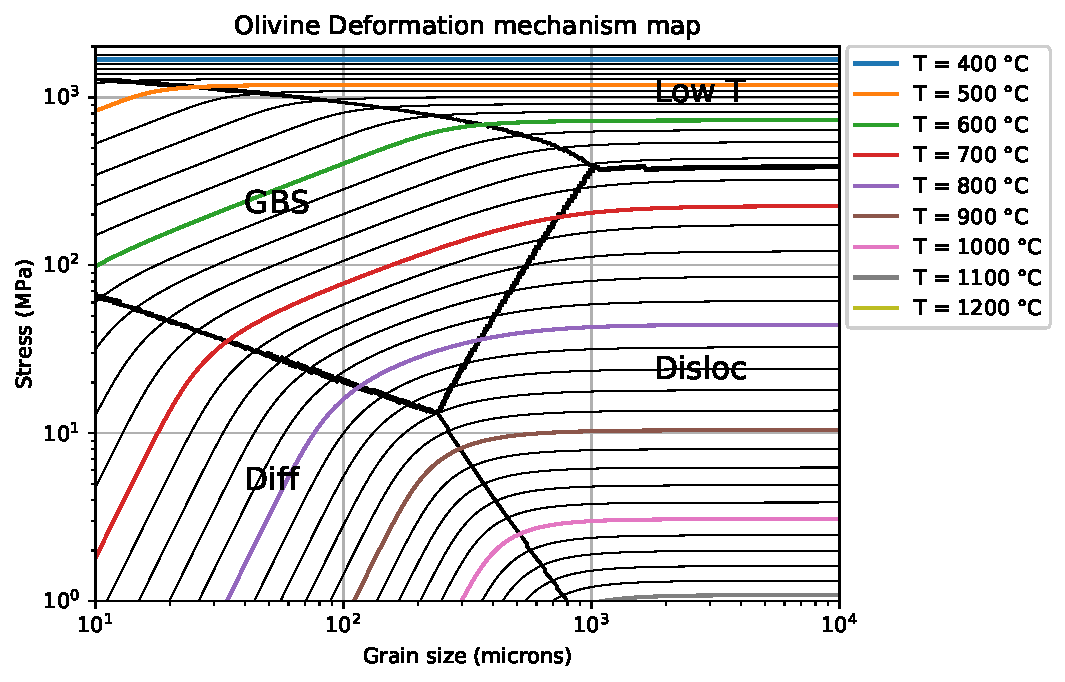
\includegraphics[width=8cm]{python_codes/fieldstone_121/results/deformation_map_boundaries_1e-15.pdf}
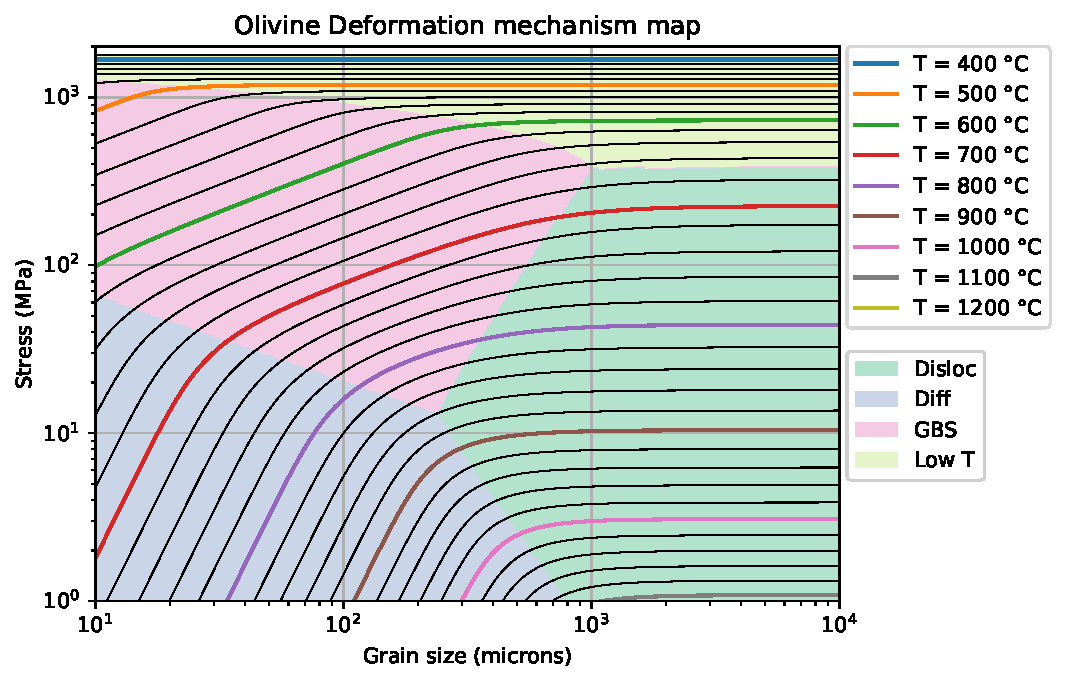
\includegraphics[width=8cm]{python_codes/fieldstone_121/results/deformation_map_filledareas_1e-15.pdf}\\
{\captionfont Deformation map as generated by the code for $\dot\varepsilon=10^{-15}~\si{\per\second}$.}
\end{center}

\begin{center}
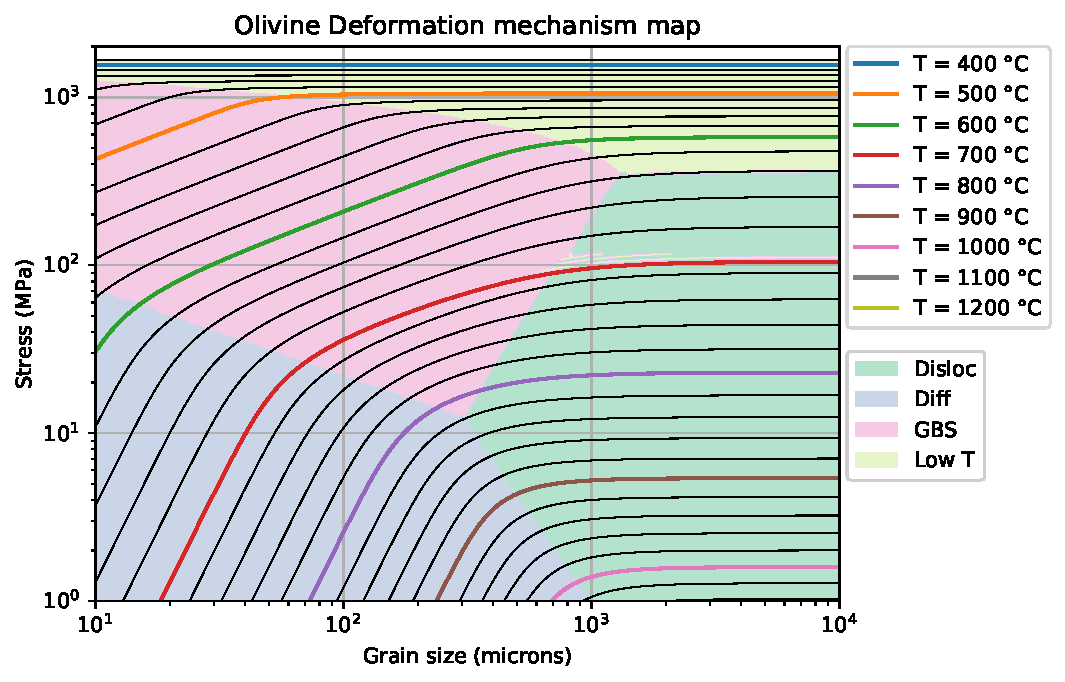
\includegraphics[width=8cm]{python_codes/fieldstone_121/results/deformation_map_filledareas_1e-16.pdf}
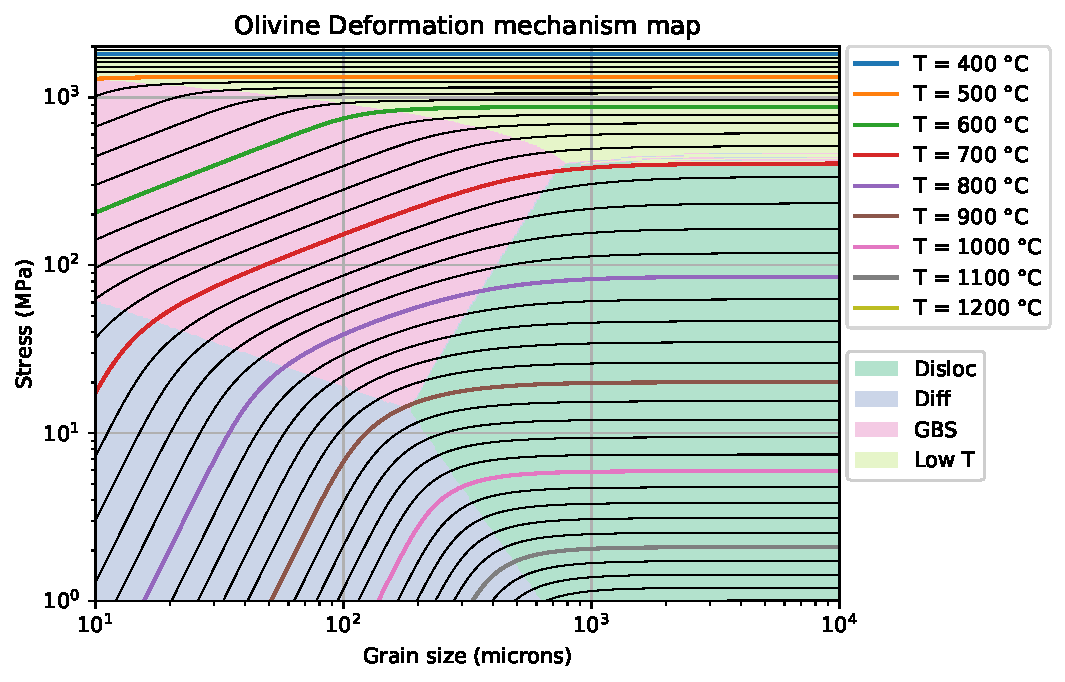
\includegraphics[width=8cm]{python_codes/fieldstone_121/results/deformation_map_filledareas_1e-14.pdf}\\
{\captionfont Deformation map as generated by the code for $\dot\varepsilon=10^{-16}~\si{\per\second}$ (left)
and $\dot\varepsilon=10^{-14}~\si{\per\second}$ (right).}
\end{center}


\begin{center}
\includegraphics[width=8cm]{python_codes/fieldstone_121/images/wahi06a}
\includegraphics[width=7cm]{python_codes/fieldstone_121/images/wahi06b}\\
{\captionfont Taken from \textcite{wahi06} (2006).
(A) An olivine deformation mechanism map, on axes of
differential stress versus grain size, contoured for strain rate, plotted
using the flow laws for dry, melt free olivine at 700C and 12 km
depth. The black recrystallization piezometer field delimits
the grain size predicted by the empirical piezometric relationship for
olivine deformed under dry conditions. The thick white
boundaries between deformation fields indicate field boundaries in the
absence of DisGBS. The thin white boundaries delineate the DisGBS
field and the dashed boundaries on either side represent uncertainty in
the location of the DisGBS boundaries due to uncertainty in its
activation energy. The change in shading within the DisGBS field
indicates the transition from the regime where creep on the easy slip
system limits the strain rate to the regime where GBS limits the strain
rate. (B) The variation of total and individual strain rates with grain
size, at a differential stress of 300 MPa, and at 700C and 12 km depth.
The dashed lines represent the individual components of DisGBS.} 
\end{center}



